% Template for PLoS
% Version 3.5 March 2018
%
% % % % % % % % % % % % % % % % % % % % % %
%
% -- IMPORTANT NOTE
%
% This template contains comments intended
% to minimize problems and delays during our production
% process. Please follow the template instructions
% whenever possible.
%
% % % % % % % % % % % % % % % % % % % % % % %
%
% Once your paper is accepted for publication,
% PLEASE REMOVE ALL TRACKED CHANGES in this file
% and leave only the final text of your manuscript.
% PLOS recommends the use of latexdiff to track changes during review, as this will help to maintain a clean tex file.
% Visit https://www.ctan.org/pkg/latexdiff?lang=en for info or contact us at latex@plos.org.
%
%
% There are no restrictions on package use within the LaTeX files except that
% no packages listed in the template may be deleted.
%
% Please do not include colors or graphics in the text.
%
% The manuscript LaTeX source should be contained within a single file (do not use \input, \externaldocument, or similar commands).
%
% % % % % % % % % % % % % % % % % % % % % % %
%
% -- FIGURES AND TABLES
%
% Please include tables/figure captions directly after the paragraph where they are first cited in the text.
%
% DO NOT INCLUDE GRAPHICS IN YOUR MANUSCRIPT
% - Figures should be uploaded separately from your manuscript file.
% - Figures generated using LaTeX should be extracted and removed from the PDF before submission.
% - Figures containing multiple panels/subfigures must be combined into one image file before submission.
% For figure citations, please use "Fig" instead of "Figure".
% See http://journals.plos.org/plosone/s/figures for PLOS figure guidelines.
%
% Tables should be cell-based and may not contain:
% - spacing/line breaks within cells to alter layout or alignment
% - do not nest tabular environments (no tabular environments within tabular environments)
% - no graphics or colored text (cell background color/shading OK)
% See http://journals.plos.org/plosone/s/tables for table guidelines.
%
% For tables that exceed the width of the text column, use the adjustwidth environment as illustrated in the example table in text below.
%
% % % % % % % % % % % % % % % % % % % % % % % %
%
% -- EQUATIONS, MATH SYMBOLS, SUBSCRIPTS, AND SUPERSCRIPTS
%
% IMPORTANT
% Below are a few tips to help format your equations and other special characters according to our specifications. For more tips to help reduce the possibility of formatting errors during conversion, please see our LaTeX guidelines at http://journals.plos.org/plosone/s/latex
%
% For inline equations, please be sure to include all portions of an equation in the math environment.  For example, x$^2$ is incorrect; this should be formatted as $x^2$ (or $\mathrm{x}^2$ if the romanized font is desired).
%
% Do not include text that is not math in the math environment. For example, CO2 should be written as CO\textsubscript{2} instead of CO$_2$.
%
% Please add line breaks to long display equations when possible in order to fit size of the column.
%
% For inline equations, please do not include punctuation (commas, etc) within the math environment unless this is part of the equation.
%
% When adding superscript or subscripts outside of brackets/braces, please group using {}.  For example, change "[U(D,E,\gamma)]^2" to "{[U(D,E,\gamma)]}^2".
%
% Do not use \cal for caligraphic font.  Instead, use \mathcal{}
%
% % % % % % % % % % % % % % % % % % % % % % % %
%
% Please contact latex@plos.org with any questions.
%
% % % % % % % % % % % % % % % % % % % % % % % %

\documentclass[10pt,letterpaper]{article}
\usepackage[top=0.85in,left=2.75in,footskip=0.75in]{geometry}

% amsmath and amssymb packages, useful for mathematical formulas and symbols
\usepackage{amsmath,amssymb}

% Use adjustwidth environment to exceed column width (see example table in text)
\usepackage{changepage}

% Use Unicode characters when possible
\usepackage[utf8x]{inputenc}

% textcomp package and marvosym package for additional characters
\usepackage{textcomp,marvosym}

% cite package, to clean up citations in the main text. Do not remove.
\usepackage{cite}

% Use nameref to cite supporting information files (see Supporting Information section for more info)
\usepackage{nameref,hyperref}

% line numbers
\usepackage[right]{lineno}

% ligatures disabled
\usepackage{microtype}
\DisableLigatures[f]{encoding = *, family = * }

% color can be used to apply background shading to table cells only
\usepackage[table]{xcolor}

% array package and thick rules for tables
\usepackage{array}


\newcommand{\cad}{---} % tiret cadratin
\newcommand{\gl}[1]{``\,#1\,''} % Guillemets standard
\newcommand{\ms}[1]{\texttt{#1}} %racccourci pour ``monospaced''
\newcommand{\lat}{\emph} %pour les mots latins

\usepackage[linesnumbered]{algorithm2e}
%\usepackage[hidelinks, colorlinks=true, linkcolor=black, citecolor=blue]{hyperref}


% create "+" rule type for thick vertical lines
\newcolumntype{+}{!{\vrule width 2pt}}

% create \thickcline for thick horizontal lines of variable length
\newlength\savedwidth
\newcommand\thickcline[1]{%
  \noalign{\global\savedwidth\arrayrulewidth\global\arrayrulewidth 2pt}%
  \cline{#1}%
  \noalign{\vskip\arrayrulewidth}%
  \noalign{\global\arrayrulewidth\savedwidth}%
}

% \thickhline command for thick horizontal lines that span the table
\newcommand\thickhline{\noalign{\global\savedwidth\arrayrulewidth\global\arrayrulewidth 2pt}%
\hline
\noalign{\global\arrayrulewidth\savedwidth}}


% Remove comment for double spacing
%\usepackage{setspace}
%\doublespacing

% Text layout
\raggedright
\setlength{\parindent}{0.5cm}
\textwidth 5.25in
\textheight 8.75in

% Bold the 'Figure #' in the caption and separate it from the title/caption with a period
% Captions will be left justified
\usepackage[aboveskip=1pt,labelfont=bf,labelsep=period,justification=raggedright,singlelinecheck=off]{caption}
\renewcommand{\figurename}{Fig}

% Use the PLoS provided BiBTeX style
\bibliographystyle{plos2015}

% Remove brackets from numbering in List of References
\makeatletter
\renewcommand{\@biblabel}[1]{\quad#1.}
\makeatother



% Header and Footer with logo
\usepackage{lastpage,fancyhdr,graphicx}
\usepackage{epstopdf}
%\pagestyle{myheadings}
\pagestyle{fancy}
\fancyhf{}
%\setlength{\headheight}{27.023pt}
%\lhead{\includegraphics[width=2.0in]{PLOS-submission.eps}}
\rfoot{\thepage/\pageref{LastPage}}
\renewcommand{\headrulewidth}{0pt}
\renewcommand{\footrule}{\hrule height 2pt \vspace{2mm}}
\fancyheadoffset[L]{2.25in}
\fancyfootoffset[L]{2.25in}
\lfoot{\today}

%% Include all macros below

\newcommand{\lorem}{{\bf LOREM}}
\newcommand{\ipsum}{{\bf IPSUM}}

%% END MACROS SECTION


\begin{document}
\vspace*{0.2in}

% Title must be 250 characters or less.
\begin{flushleft}
{\Large
\textbf\newline{Efficient similarity-based data clustering by optimal object to cluster reallocation} % Please use "sentence case" for title and headings (capitalize only the first word in a title (or heading), the first word in a subtitle (or subheading), and any proper nouns).
}
\newline
% Insert author names, affiliations and corresponding author email (do not include titles, positions, or degrees).
\\
Mathias Rossignol\textsuperscript{1\Yinyang},
Mathieu Lagrange\textsuperscript{2*\Yinyang},
Arshia Cont\textsuperscript{1\ddag} % \textcurrency
\\
\bigskip
\textbf{1} Ircam, CNRS, Paris, France
\\
\textbf{2} Ls2n, CRNS, Ecole Centrale Nantes, Nantes, France
\\
\bigskip

% Insert additional author notes using the symbols described below. Insert symbol callouts after author names as necessary.
%
% Remove or comment out the author notes below if they aren't used.
%
% Primary Equal Contribution Note
\Yinyang These authors contributed equally to this work.

% Additional Equal Contribution Note
% Also use this double-dagger symbol for special authorship notes, such as senior authorship.
\ddag This author contributed to the writing of the manuscript.

% Current address notes
%\textcurrency Current Address: Dept/Program/Center, Institution Name, City, State, Country % change symbol to "\textcurrency a" if more than one current address note
% \textcurrency b Insert second current address
% \textcurrency c Insert third current address

% Group/Consortium Author Note
%\textpilcrow Membership list can be found in the Acknowledgments section.

% Use the asterisk to denote corresponding authorship and provide email address in note below.
* mathieu.lagrange@cnrs.fr
\end{flushleft}
% Please keep the abstract below 300 words
\section*{Abstract}
We present an iterative flat hard clustering algorithm designed to operate on arbitrary similarity matrices, with the only constraint that these matrices be symmetrical. Although functionally very close to kernel k-means, our proposal performs a maximization of average intra-class similarity, instead of a squared distance minimization, in order to remain closer to the semantics of similarities. We show that this approach permits the relaxing of some conditions on usable affinity matrices like semi-positiveness, as well as opening possibilities for computational optimization required for large datasets. Systematic evaluation on a variety of data sets shows that compared with kernel k-means and the spectral clustering methods, the proposed approach gives equivalent or better performance, while running much faster. Most notably, it significantly reduces memory access, which makes it a good choice for large data collections. Material enabling the reproducibility of the results is made available online.

\linenumbers


%\keywords{clustering, similarity, non-metric data representation, time series clustering}

\section*{Introduction}

Clustering collections of objects into classes that bring together similar ones is probably the most common and intuitive tool used both by human cognition and artificial data analysis in an attempt to make that data organized, understandable, manageable. When the studied objects lend themselves to this kind of analysis, it is a powerful way to expose underlying organizations and approximate the data in such a way that the relationships between its members can be statistically understood and modeled. Given a description of objects, we first attempt to quantify which ones are ``\,similar\,'' from a given point of view, then group those $n$ objects into $C$ clusters, so that the similarity between objects within the same cluster is maximized. Finding the actual best possible partition of objects into clusters is, however, an NP-complete problem, intractable for useful datasets sizes. Many approaches have been proposed to yield an approximate solution: analytic, iterative, flat or hierarchical, agglomerative or divisive, soft or hard clustering algorithms, \textit{etc.}, each with their strengths and weaknesses \cite{jain2010data}, performing better on some classes of problems than others \cite{steinbach2000comparison,thalamuthu2006evaluation}.

Iterative divisive hard clustering algorithms, usually perform well to identify high-level organization in large data collections in reasonable running time. For that reason, they are a sensible choice in many data mining situations, and constitute our focus in this paper.
% ; their main drawback being that the number of desired clusters must be specified
If the data lies in a vector space, \textit{i.e.} an object can be described by a $m$-dimensional feature vector without significant loss of information, the seminal \emph{k-means} algorithm \cite{macQueenBsmsp67} is probably the most efficient approach, since the explicit computation of the cluster centroids ensure both computational efficiency and scalability. This algorithm is  based on the centroid model, and minimizes the intra cluster Euclidean distance. As shown by \cite{Banerjee:2005:CBD:1046920.1194902}, any kind of Bregman divergence, such as the KL-divergence \cite{Dhillon:2003:DIT:944919.944973} or the Itakura-Saito divergence \cite{linde:algorithm}, may also be considered to develop such efficient clustering algorithms.

However, for many types of data, the projection of a representational problem into an vector space cannot be done without significant loss of descriptive efficiency. To reduce this loss, specifically tailored measures of similarity are considered. As a result, the input data for clustering is no longer a $n \times m$ matrix storing the $m$-dimensional vectors describing the objects, but a (usually symmetric) square matrix $S$ of size $n \times n$ which numerically encodes some sort of relationship between the objects. In this case, one has to resort to clustering algorithms based on connectivity models, since the cluster centroids cannot be explicitly computed.

Early attempts to solve this issue considered the k-medoids problem, where the goal is to find the $k$ objects that maximize the average similarity with the other objects of their respective clusters, or \emph{medoids}. The Partition Around Medoids (PAM) algorithm \cite{KaufmanRousseeuw90} solves the k-medoids problem but with a complexity of $O(k(n-k)^2)i$, $n$ being the number of objects and $i$ number of iterations. Due to the high complexity and the low convergence rate, this algorithm cannot be applied to decent size datasets. In order to scale the approach, the Clustering LARge Applications (CLARA) algorithm \cite{KaufmanRousseeuw90} draws a sample of objects before running the PAM algorithm. This sampling operation is repeated several times and the most satisfying set of medoids is retained. In contrast, CLARANS \cite{Ng:1994:EEC:645920.672827} preserves the whole set of objects but cuts complexity by  drawing a sample of neighbors in each search for the medoids.
%, with two drawbacks: it assumes that all objects fit in main memory, and the result is sensitive to the input order \cite{Zhang:1996:BED:233269.233324}.


Another classical approach to the issue is to run a variant of k-means that considers average intra-cluster similarity as the guiding criterion for object-to-class reallocation \cite[Chapter 10.7]{Duda01}. This straightforward technique performs well in many cases, but the complexity of computing anew intra-cluster similarities at each iteration makes it impractical for large datasets.

Following work on kernel projection \cite{Vapnik:1995:NSL:211359}, that is, the fact that a nonlinear data transformation into some high dimensional feature space increases the probability of the linear separability of patterns within the transformed space, \cite{Girolami:2002:MKC:2325785.2326903} introduced a kernel version of the K-means algorithm, whose input is a kernel matrix $\mathcal{K}$ that must be a Gram matrix, \textit{i.e.} semi definite positive. \cite{Dhillon:2007:WGC:1313055.1313291} linked a weighted version of the kernel K-means objective to the popular spectral clustering \cite{von2007tutorial}, introducing an efficient way of solving the normalized cut objective \cite{shi2000normalized}.

The kernel k-means algorithm proves to be equally useful when considering arbitrary similarity problems if special care is taken to ensure definite positiveness of the input matrix \cite{Roth:2003:OCP:960254.960291}. This follows original algorithmic considerations where vector space data is projected into high dimensional spaces using a carefully chosen kernel function.

%% Long sentence! rewritten above
%Originally thought as considering data lying initially in a given vector space then projected in an high dimensional features space thanks to a carefully chosen kernel function, the kernel k-means algorithm proved to be equally useful when considering arbitrary similarity problems if some special care is taken to ensure definite positiveness of the input matrix (\cite{Roth:2003:OCP:960254.960291}).

Despite such improvements, kernel k-means cannot be easily applied to large scale datasets without special treatments because of high algorithmic and memory access costs.
%Still, the complexity of the algorithm and the cost of memory  access  prevent from using the kernel k-means algorithm for large scale datasets without specific treatments.
\cite{Chitta:2011:AKK:2020408.2020558} considered sampling of the input data, \cite{1047453} considered block storing of the input matrix, and a pre-clustering  approach \cite{bradley98scaling} is considered by \cite{Kulis2008} with a coarsening and refining phases as respectively a pre- and post-treatment of the actual clustering phase.

We show in this paper that by using a semantically equivalent variant of the average intra-cluster similarity presented in \cite[Chapter 10.7]{Duda01}, it becomes possible to perform a computationally efficient greedy optimization \cite[Chapter 10.8]{Duda01} with guaranteed convergence for arbitrary similarity measures. Although both of those techniques are well known, combining them is non trivial, and lead to a clustering algorithm, which we call k-averages with the following properties:
\begin{itemize}
\item input data can be arbitrary symmetric similarity matrices,
\item it has fast and guaranteed convergence, with a number of object to clusters reallocations experimentally found to be roughly equal to the number of objects,
\item it provides good scalability thanks to a reduced need for memory access, and
\item on a collection of synthetic and natural test data, its results are equivalent to those of kernel k-means, and obtained in a fraction of its computing time, particularly when paged memory is required.
\end{itemize}

To summarize, the main contribution of the paper is to present a clustering algorithm:
\begin{itemize}
  \item  that can handle arbitrary affinity matrices, \textit{i.e.} semi-positiveness is not a mandatory requirement for guaranteed convergence
  \item thanks to a carefully designed strategy to update the membership of objects to cluster, the algorithm is fast and memory efficient.
\end{itemize}

The remaining of the paper is organized as follows: Section~\ref{sec:kkmeans} presents the kernel k-means objective function and the basic algorithm that minimizes this function, and Section~\ref{sec:kaverages} introduces the concepts behind the k-averages algorithm,
%before giving a detailed description of it in Section~\ref{sec:algo}.
followed by a detailed algorithmic description in Section~\ref{sec:algo}.
The complexity of the two algorithms in terms of arithmetic operations and memory access is then studied in Section \ref{sec:complexity}. The above presented properties of the proposed k-averages algorithm are then validated on synthetic controlled data in Section \ref{sec:validation} and on 43 datasets of time series issued from various sources in Section \ref{sec:experiments}.

\section{Kernel k-means} \label{sec:kkmeans}

Since its introduction by \cite{Girolami:2002:MKC:2325785.2326903}, kernel k-means has been an algorithm of choice for flat data clustering with known number of clusters \cite{Kulis2008, Roth:2003:OCP:960254.960291}. It makes use of a mathematical technique known as the \gl{kernel trick} to extend the classical k-means clustering algorithm \cite{macQueenBsmsp67} to criteria beyond simple euclidean distance proximity. Since it constitutes the closest point of comparison with our own work, we dedicate this section to its detailed presentation.

In the case of kernel k-means, the kernel trick allows us to  consider that the k-means algorithm is operating in an unspecified, possibly very high-dimensional Euclidean space; but instead of specifying the properties of that space and the coordinates of objects, the equations governing the algorithm are modified so that everything can be computed knowing only the scalar products between points. The symmetrical matrix  containing those scalar products is known as a kernel, noted $\mathcal{K}$.

\subsection{Kernel k-means objective function}

In this section and the following, we shall adopt the following convention: $N$ is the number of objects to cluster and $C$ the number of clusters; $N_c$ is the number of objects in cluster $c$, and $\mu_c$ is the centroid of that cluster. $z_{cn}$ is the membership function, whose value is $1$ if object $o_n$ is in class $c$, $0$ otherwise. In the folowing equations, $\mu_c$ and $o_n$ are assumed to be column vectors of equal dimension.

Starting from the objective function minimized by the k-means algorithm, expressing the sum of squared distances of points to the centroids of their respective clusters:

\[
S = \sum_{c=1}^{C} \sum_{n=1}^{N} z_{cn} \left(o_n-\mu_c\right)^\top\left(o_n-\mu_c\right) \label{eq:S}
\]

And using the definition of centroids as:

\[
\mu_c = \frac{1}{N_c}\sum_{n=1}^{N}z_{cn}o_n
\]

$S$ can be developed and rewritten in a way that does not explicitly refer to the centroid positions, since those cannot be computed:

\[
S = \sum_{c=1}^{C} \sum_{n=1}^{N} z_{cn} Y_{cn}
\]

where
\begin{align}
\begin{split}
Y_{cn} & =  \left(o_n-\mu_c\right)^\top\left(o_n-\mu_c\right) \\
       & =  o_no_n - 2 o_n^\top \mu_c + \mu_c^\top \mu_c \\
       & =  o_n^\top o_n - 2 o_n^\top \frac{1}{N_c} \sum_{i=1}^{N} z_{ci} o_i +
       	 \left(\frac{1}{N_c} \sum_{i=1}^{N} z_{ci} o_i\right)^\top
         \left(\frac{1}{N_c} \sum_{i=1}^{N} z_{ci} o_i\right)\\
        %  \left(\frac{1}{N_c} \sum_{i=1}^{N} z_{ci} o_i\right)^2\\ %.\left(\frac{1}{N_c} \sum_{i=1}^{N} z_{ci} o_i\right) \\
       & =  o_n^\top o_n - \frac{2}{N_c} \sum_{i=1}^{N} z_{ci} o_n^\top o_i +
       	 \frac{1}{N_c^2} \sum_{i=1}^{N} \sum_{j=1}^{N} z_{ki} z_{kj} o_i^\top o_j \\
       & =  \mathcal{K}_{nn} - \frac{2}{N_c} \sum_{i=1}^{N} z_{ci} \mathcal{K}_{ni} +
         \frac{1}{N_c^2} \sum_{i=1}^{N} \sum_{j=1}^{N} z_{ki} z_{kj} \mathcal{K}_{ij} \label{eq:yki}
\end{split}
\end{align}

%\begin{eqnarray}
%Y_{cn} & = & \left(o_n-\mu_c\right)\left(o_n-\mu_c\right)^\top \\
%       & = & o_n.o_n - 2 o_n.\mu_c + \mu_c.\mu_c \\
%       & = & o_n.o_n - 2 o_n.\frac{1}{N_c} \sum_{i=1}^{N} z_{ci} o_i +
%       	 \left(\frac{1}{N_c} \sum_{i=1}^{N} z_{ci} o_i\right).\left(\frac{1}{N_c} \sum_{i=1}^{N} z_{ci} o_i\right) \\
%       & = & o_n.o_n - \frac{2}{N_c} \sum_{i=1}^{N} z_{ci} o_n.o_i +
%       	 \frac{1}{N_c^2} \sum_{i=1}^{N} \sum_{j=1}^{N} z_{ki} z_{kj} o_i.o_j \\
%       & = & \mathcal{K}_{nn} - \frac{2}{N_c} \sum_{i=1}^{N} z_{ci} \mathcal{K}_{ni} +
%         \frac{1}{N_c^2} \sum_{i=1}^{N} \sum_{j=1}^{N} z_{ki} z_{kj} \mathcal{K}_{ij} \label{eq:yki}
%\end{eqnarray}

%% Comment by Arshia: The following paragraph is too fast!
% what does "mostly bounded" mean?
% The second half going to "similarity matrix processing" can be further explained.. this means that K_nn will become similarity measures.. right?

Since the sum of $K_{nn}$ over all points remains constant, and the sum of squared centroid norms (third, quadratic, term of Equation~\ref{eq:yki}) is mostly bounded by the general geometry of the cloud of objects, we can see that minimizing this value implies maximizing the sum of the central terms, which are the average scalar products of points with other points belonging to the same class. Therefore, given a matrix gathering similarities between objects, if that matrix possesses the necessary properties to be considered as a kernel (positive semidefinitness), then the kernel k-means algorithm can be applied to it in order to create clusters that locally maximize the average intra-cluster similarity.

\subsection{Algorithm}

Finding the configuration that globally minimizes S (Eq.~\ref{eq:S}) is an NP-complete problem. However, several approaches allow finding an acceptable approximation. We shall only focus here on the fastest and most popular, an iterative assignment\,/\,update procedure commonly referred to as the \gl{k-means algorithm} \cite{macQueenBsmsp67}, or as a discrete version of Lloyd's algorithm, detailed in Algorithm~\ref{algo:kkmeans}.

\begin{algorithm}
	\SetAlgoLined
	\KwData{number of objects $N$, number of classes $C$, kernel matrix $\mathcal{K}$}
	\KwResult{label vector $L$ defining a partition of the objects into $C$ classes}
	\BlankLine
	\textbf{Initialization:} fill L with random values in $[1..C]$\;
	\BlankLine
	\While {$L$ is modified} {
		\For {$n \leftarrow 1$ to $N$} {
			\For {$c \leftarrow 1$ to $C$} {
				Compute $Y_{cn}$ following Eq.~\ref{eq:yki} \label{algline:kkmeans_cplx1}
				(note: $z_{cn} = (L_n == c)\,?\,1\;:\;0$)
			}
			$L_n = \textrm{argmin}_c (Y_{cn})$\;
		}
	}
	\BlankLine
	\caption{Lloyd's algorithm applied to minimizing the kernel k-means objective.}
  \label{algo:kkmeans}
\end{algorithm}

The version given here is the most direct algorithmic translation of the mathematical foundations developed above, and as we shall see in section~\ref{sec:complexity}, it can easily become more efficient. Before that, we introduce our proposed k-averages algorithm.


\section{Foundations of the k-averages algorithm} \label{sec:kaverages}

In our proposal, we adopt an alternative objective function which, unlike kernel k-means, does not rely on a geometric interpretation but an explicit account of the similarity matrix. The goal is to maximize the average intra-cluster similarity between points, a commonly used metric to evaluate clustering quality, and one whose computation is direct\cad{}linear in time.

Due to its simplicity, however, the objective function cannot be simply \gl{plugged into} the standard kernel k-means algorithm: it lacks the geometric requisites to ensure convergence. We must therefore propose a specifically tailored algorithmic framework to exploit it: first, we show here that it is possible to easily compute the impact on the global objective function of moving a single point from one class to another; this allows us to develop a greedy optimization algorithm taking advantage of that formula.

\subsection{Conventions and objective function}

In addition to the notations presented above, we index here the set of elements belonging to a given cluster $c_k$ as $c_k = \left\{o_{k1}, \ldots, o_{kN_k}\right\}$.
For simplicity, we omit the first index and note $c = \left\{o_1, \ldots, o_{N_c}\right\}$ when considering a single class.
%To simplify below, when we're simply considering one class, no matter
%which, we shall omit the first index and write $c = \left\{o_1, \ldots, o_{N_c}\right\}$.

The similarity between objects shall be written $s\left(o_i, o_j\right)$.
%Let us
We extend the notation $s$ to the \emph{similarity of an object to a
  class} defined as the average similarity of an object
with all objects of the class. $s(o,c)$ accepts two definitions,
depending on whether or not $o$ is a member of $c$:

If $o \notin c$,
\begin{equation}
  s\left(o,c\right) = \frac{1}{N_c} \sum_{i=1}^{n_c}s\left(o, o_i\right)
   \label{eq:soc_notinclass}
\end{equation}

If $o \in c$, then necessarily $\exists i \mid o = o_i$
\begin{equation}
  s\left(o,c\right) = s\left(o_i, c\right) = \frac{1}{N_c-1} \sum_{j=1 \ldots n_c, j \neq i} s\left(o_i, o_j\right)
  	 \label{eq:soc_inclass}
\end{equation}

Let us call the \gl{quality} of a class the average intra-class object-to-object similarity, and write it $\mathcal{Q}$:
\begin{equation}
	\mathcal{Q}\left(c\right) = \frac{1}{N_c} \sum_{i=1}^{n_c} s\left(o_i, c\right)
    \label{eq:class_qual_base}
\end{equation}

%Indeed, we never refer to a geometrical interpretation of the data. However, it should be noted that since in k-means (and kernel k-means) the centroid of a class is defined as an average of all points in that class, $\mathcal{Q}$ is strictly equivalent to the average point to centroid similarity.

In our framework, we do not explicitly refer to class centroids, preferring to directly consider averages of similarity values between individuals within clusters. Using the notations above, we define our objective function as the average class quality, normalized with class sizes:

\begin{equation}
  \mathcal{O} = \frac{1}{N} \sum_{i=1}^{C} N_i \mathcal{Q}(c_i)
  \label{eq:objective_function}
\end{equation}

Since, informally, our goal is to bring together objects that share high similarity, a first idea would be to simply repeatedly move each object to the class with whose members it has the highest average similarity. This is what we call the \gl{naive k-averages} algorithm.

\subsection{Naive k-averages algorithm}

Algorithm~\ref{algo:naive-kaverages} presents a method that simply moves each object to the class with which it has the highest average similarity, until convergence is reached. The algorithm is straightforward and simple; however, experiments show that while it can often produce interesting results, it also sometimes cannot reach convergence because the decision to move an object to a different cluster is taken without considering the impact of the move on the quality of the source cluster.

\begin{algorithm}
	\SetAlgoLined
	\KwData{number of objects $N$, number of classes $C$, similarity matrix $\mathcal{S}$}
	\KwResult{label vector $L$ defining a partition of the objects into $C$ classes}
	\BlankLine
	\textbf{Initialization:}
		Fill L with random values in $[1..C]$\;
		Compute initial object-class similarities $S$ following Eq.~\ref{eq:soc_inclass} or Eq.~\ref{eq:soc_notinclass}\;
	\BlankLine
	\While {$L$ is modified} {
		\For {$i \leftarrow 1$ to $N$} {
			previousClass $\leftarrow L_i$\;
			nextClass $\leftarrow \mathrm{argmin}_k\, S(i, k)$
			\If {nextClass $\ne$ previousClass} {
				$L_i \leftarrow \mathrm{nextClass}$\;
				\For {$j \leftarrow 1$ to $N$}{
					Update $S(j,nextClass)$ and $S(j,previousClass)$
				}
			}
		}
	}
	\BlankLine
	\caption{The naive k-averages algorithm.}
  \label{algo:naive-kaverages}
\end{algorithm}

To ensure convergence, we need to compute the impact on the objective function of moving one object from one class to another. Using such formulation and performing only reallocation that have a positive impact, the convergence of such an iterative algorithm is guaranteed.

\subsection{Impact of object reallocation on class quality}

Considering a class $c$, let us develop the expression of $\mathcal{Q}(c)$ into a more useful form. Since all objects are in $c$, we use the formula in (Eq.~\ref{eq:soc_inclass}) to get:

\begin{equation*}
  \begin{aligned}
    \mathcal{Q}\left(c\right) & = \frac{1}{N_c} \sum_{i=1}^{N_c} \frac{1}{N_c-1} \sum_{\substack{j=1 \ldots N_c\\j \neq i}} s\left(o_i, o_j\right) \\
                              & = \frac{1}{N_c(N_c-1)} \sum_{i=1}^{N_c} \sum_{\substack{j=1 \ldots N_c\\j \neq i}} s\left(o_i, o_j\right)
  \end{aligned}
\end{equation*}

Using the assumption that the similarity matrix is symmetrical, we can reach: % (this is an indispensable transformation for future calculations):
\begin{equation}
    \mathcal{Q}\left(c\right) = \frac{2}{N_c(N_c-1)} \sum_{i=2}^{N_c} \sum_{j=1}^{i-1} s\left(o_i, o_j\right)
    \label{eq:classQuality}
\end{equation}

For future use and given the importance of the above transformation, we define:
\[
  \Sigma(c) = \sum_{i=2}^{N_c} \sum_{j=1}^{i-1} s\left(o_i, o_j\right)
\]

Thus:
\[
\mathcal{Q}\left(c\right) = \frac{2}{N_c(N_c-1)}\Sigma(c) \phantom{XX}\mathrm{and}\phantom{XX} \Sigma(c) = \frac{N_c(N_c-1)\mathcal{Q}\left(c\right)}{2}
\]

\subsubsection{Removing an object from a class}

Assuming that $o \in c$, necessarily $\exists i \mid o=o_i$. Since the numbering of objects is arbitrary, we can first simplify the following equation by considering that $o = o_{N_c}$, in order to reach a formula that is independent from that numbering.

\begin{equation*}
  \begin{aligned}
    \mathcal{Q}\left(c \smallsetminus o_{N_c}\right) & = \frac{2}{(N_c-1)(N_c-2)} \sum_{i=2}^{N_c-1} \sum_{j=1}^{i-1} s\left(o_i, o_j\right) \\
                                                   & = \frac{2}{(N_c-1)(N_c-2)} \left[\Sigma(c) - \sum_{j=1}^{N_c-1} s\left(o_{N_c}, o_j\right) \right] \\
                                                   & = \frac{2}{(N_c-1)(N_c-2)} \left[\Sigma(c) - (N_c-1)s\left(o_{N_c}, c\right) \right] \\
                                                   & = \frac{2N_c(N_c-1)\mathcal{Q}(c)}{2(N_c-1)(N_c-2)} - \frac{2(N_c-1)s\left(o_{N_c}, c\right)}{(N_c-1)(N_c-2)}\\
                                                   & = \frac{N_c \mathcal{Q}(c)  - 2s\left(o_{N_c}, c\right)}{N_c-2}
  \end{aligned}
\end{equation*}

The quality of a class after removal of an object is thus:

\begin{equation}
  \mathcal{Q}\left(c \smallsetminus o\right) = \frac{N_c \mathcal{Q}(c)  - 2s\left(o, c\right)}{N_c-2}
  \label{eq:newQual_remove}
\end{equation}

And the change in quality from its previous value:

\begin{equation} \label{deltaRemove}
  \begin{aligned}
    \mathcal{Q}\left(c \smallsetminus o\right) - \mathcal{Q}\left(c\right) & = \frac{N_c \mathcal{Q}(c)  - (N_c-2) \mathcal{Q}(c)  - 2s\left(o, c\right)}{N_c-2} \\
                                                                           & = \frac{2\left( \mathcal{Q}(c) - s\left(o, c\right)\right)}{N_c-2}
    \end{aligned}
\end{equation}


\subsubsection{Adding an object to a class}

Assuming that $o \notin c$, we can similarly to what has been done previously (numbering is arbitrary) consider for the sake of simplicity that $o$ becomes $o_{N_c+1}$ in the modified class $c$. Following a path similar to above, we get:

\begin{equation*}
  \begin{aligned}
    \mathcal{Q}(c \cup o_{N_c+1}) & = \frac{2}{N_c(N_c+1)} \sum_{i=2}^{N_c+1} \sum_{j=1}^{i-1} s\left(o_i, o_j\right) \\
                                & = \frac{2}{N_c(N_c+1)} \left[\Sigma(c) + N_c s\left(o_{N_c+1}, c\right)\right] \\
                                & = \frac{(N_c-1) \mathcal{Q}(c)  + 2s\left(o_{N_c+1}, c\right)}{N_c+1}
  \end{aligned}
\end{equation*}

\noindent The quality of a class $c$ after adding an object $o$ is thus:

\begin{equation}
  \mathcal{Q}\left(c \cup o\right) = \frac{(N_c-1) \mathcal{Q}(c)  + 2s\left(o, c\right)}{N_c+1}
  \label{eq:newQual_add}
\end{equation}

\noindent And the change in quality from its previous value:

\begin{equation} \label{deltaAdd}
    \mathcal{Q}\left(c \cup o\right) - \mathcal{Q}\left(c\right)  = \frac{2\left(s\left(o, c\right)-\mathcal{Q}(c)\right)}{N_c+1}
\end{equation}

%\begin{equation} \label{deltaAdd}
%  \begin{aligned}
%    \mathcal{Q}\left(c \cup o\right) - \mathcal{Q}\left(c\right) & = \frac{(N_c-1) \mathcal{Q}(c)  - (N_c+1) \mathcal{Q}(c)  + 2s\left(o, c\right)}{N_c+1} \\
%                                                                           & = \frac{2\left(s\left(o, c\right)-\mathcal{Q}(c)\right)}{N_c+1}
%    \end{aligned}
%\end{equation}

\subsection{Impact of object reallocation on the global objective function}
\label{sec:delta_definition}

When moving an object $o$ from class $c_s$ (\gl{source}), to whom it belongs, to a
distinct class $c_t$ (\gl{target}), $(N_s-1)$ objects are affected
by the variation in (\ref{deltaRemove}), and $N_t$ are affected
by that in (\ref{deltaAdd}); in addition, one object $o$ moves from a class whose quality is $\mathcal{Q}(c_s)$ to one whose quality is $\mathcal{Q}\left(c_t \cup o\right)$, as expressed by Eq.~\ref{eq:newQual_add}, which leads to an impact of moving object $o$ from class $c_s$ to class $c_t$ wich can be computed as follows:

\begin{align}
\begin{split}
  \delta_o(c_s, c_t) = & \frac{2N_t \left(s\left(o, c_t\right)-\mathcal{Q}(c_t)\right)}{N_t+1} + \\
&  \frac{2(N_s-1)\left( \mathcal{Q}(c_s) - s\left(o, c_s\right)\right)}{N_s-2}  + \\
 &  \frac{(N_t-1) \mathcal{Q}(c_t)  + 2s\left(o, c_t\right)}{N_t+1} - \mathcal{Q}(c_s) \\
\end{split}
  \label{eq:impact_classnorm}
\end{align}

As can be seen, computing this impact is a fixed-cost operation. We can therefore use the formula as the basis for an efficient iterative algorithm.

\section{K-averages algorithm}
\label{sec:algo}

\begin{algorithm}[h!]
	\SetAlgoLined
	\KwData{number of objects $N$, number of classes $C$, similarity matrix $\mathcal{S}$}
	\KwResult{label vector $L$ defining a partition of the objects into $C$ classes}
	\BlankLine
	\textbf{Initialization:}
		Fill L with random values in $[1..C]$\;
		Compute initial object-class similarities $S$ following Eq.~\ref{eq:soc_inclass} or Eq.~\ref{eq:soc_notinclass}\;
		Compute initial class qualities $\mathcal{Q}$ following Eq.~\ref{eq:classQuality}\;
	\BlankLine
	\While {$L$ is modified} {
		\For {$i \leftarrow 1$ to $N$} {
			previousClass $\leftarrow L_i$\;
			nextClass $\leftarrow \mathrm{argmax}_k\,\delta_i(\mathrm{previousClass}, k)$ \label{algline:kaverages_search}
			(following the definition of $\delta$ in Eq.~\ref{eq:impact_classnorm})\; % Eq.~\ref{eq:impact_objnorm} or
			\If {nextClass $\ne$ previousClass} {
				$L_i \leftarrow \mathrm{nextClass}$\;
				Update $\mathcal{Q}_\mathrm{previousClass}$ following Eq.~\ref{eq:newQual_remove}\;
				Update $\mathcal{Q}_\mathrm{nextClass}$ following Eq.~\ref{eq:newQual_add}\;
				\For {$j \leftarrow 1$ to $N$}{
					Update $S(j,nextClass)$ and $S(j,previousClass)$ \label{algline:kaverages_recompute} \\ following Eq.~\ref{eq:newSimilNewC}\;
				}
			}
		}
	}
	\BlankLine
	\caption{The K-averages algorithm.}
  \label{algo:kaverages}
\end{algorithm}

Our approach does not allow us to benefit, like kernel k-means, from the convergence guarantee brought by the geometric foundation of k-means. In consequence, we cannot apply a \gl{batch} approach where at each iteration all elements are moved to their new class, and all distances (or similarities) are computed at once. To guarantee convergence, we must update the class properties for the two modified classes (source and destination), as well as recompute the average class-object similarities for them for each considered object, after finding its ideal new class. This is the principle of the \gl{greedy} k-means algorithm \cite[Chapter10.8]{Duda01}, but whereas for k-means that approach increases complexity (and even more so for kernel k-means), in this case it leads to a much improved computational performance.

Indeed, at a first glance, dynamically updating objectives as a result of object reallocation might seem to have negative performance impact. However, our simple non-quadratic updates make such dynamic changes easily tractable. New class qualities are thus given by eqs.~\ref{eq:newQual_remove} and \ref{eq:newQual_add}, and new object-class similarities can be computed by:

%% Rewritten above.. feel free to modify!!! (Arshia)
%Although this seems at first like systematically updating everything at each object re-allocation should have a huge performance impact, our reliance on simple averages without any quadratic terms makes it possible to have very simple update formulas: new class qualities are given by Equations~\ref{eq:newQual_remove} and \ref{eq:newQual_add}, and new object-class similarities can be computed by:

\begin{equation}
	\begin{aligned}
    s(i, c_s(t+1)) &= \frac{N_s(t).s(i, c_s(t)) + s(i,n)}{N_s(t)+1} \\
    s(i, c_t(t+1)) &= \frac{N_t(t).s(i, c_s(t)) - s(i,n)}{N_t(t)-1}
   	\end{aligned}
  \label{eq:newSimilNewC}
\end{equation}

\noindent where $i$ is any object index, $n$ is the recently reallocated object, $c_s$ the \gl{source} class that object $i$ was removed from, and $c_t$ the \gl{target} class that object $n$ was added to.

The full description of k-averages is given in Algorithm~\ref{algo:kaverages}.

\section{Convergence}
\label{sec:convergence}

The kernel k-means algorithm ensures convergence if the similarity matrix is semi-definite positive. The k-averages algorithm relaxes this constraint by only requiring symmetricity of the similarity matrix to ensure convergence.

An algorithm is guaranteed to converge if its successive iterations can be tied to a strictly monotonous and bounded quantity. For the k-averages algorithm, this quantity is the objective function itself, as we now show.

Thanks to the rewriting of the class quality function done in Eq.~\ref{eq:classQuality}, which only requires the similarity matrix to be symmetrical, we can directly define the allocation decision criterion $\delta$ (Eq.~\ref{eq:impact_classnorm}) to be the change in the global objective function $\mathcal{O}$ (Eq.~\ref{eq:objective_function}) implied by reallocating an object to a new class. It follows that, as long as reallocations are only performed when $\delta > 0$, $\mathcal{O}$ is strictly increasing throughout the execution of the algorithm.

Moreover, $\mathcal{O}$, defined as a weighted average of the average intra-class similarities for the produced clusters, can be proven to never exceed the maximal similarity between two objects.

Indeed, the average similarity of an object to other members of its class, expressed as $s(o,c)$ in Eq.~\ref{eq:soc_notinclass}, is an average of similarities, and therefore lower than or equal to their maximum value. Similarly, the quality $\mathcal{Q}$ of a class, defined as the average of object to class similarities (Eq.~\ref{eq:class_qual_base}), is inferior to the maximum value of $s(o,c)$, and therefore to the maximum similarity between objects. Finally, $\mathcal{O}$, a weighted average of $\mathcal{Q}$ values, is, once again, inferior to their maximum value.

The objective function $\mathcal{O}$ is thus upper-bounded, and increases at each iteration of the outer loop of Algorithm~\ref{algo:kaverages}; which guarantees its convergence.

\section{Complexity analysis}
\label{sec:complexity}

In this section, we study the complexity of the two approaches presented above, first from the point of view of raw complexity, second by focusing on memory access.

\subsection{Computational complexity}

\subsubsection{Kernel k-means}

As can be seen in Algorithm~\ref{algo:kkmeans}, the operation on line~\ref{algline:kkmeans_cplx1} is the most costly part of the algorithm: for each object $n$ and class $c$, at each iteration, it is necessary to compute $Y_{cn}$ from Eq.~\ref{eq:yki}\cad{}an $O(N^2)$ operation in itself, per object. The impossibility of simply computing the distances to a known centroid as done in the k-means algorithm leads to a much higher complexity for the kernel k-means algorithm, globally $O(N^3)$ per iteration, independent of how many objects are moved for that iteration.

It is however possible to improve the performance of kernel k-means by noting than in Eq.~\ref{eq:yki}, the third term of the equation, which has the highest complexity, is only dependent on class definitions and not on the considered object. We can therefore rewrite Eq.~\ref{eq:yki} as:

\begin{eqnarray}
Y_{cn} & = & \mathcal{K}_{nn} - \frac{2}{N_c} \sum_{i=1}^{N} z_{ci} \mathcal{K}_{ni} + M_c \label{eq:yki_improved}
\end{eqnarray}
where
\begin{eqnarray}
M_c    & = & \frac{1}{N_c^2} \sum_{i=1}^{N} \sum_{j=1}^{N} z_{ki} z_{kj} \mathcal{K}_{ij} \label{eq:mc}
\end{eqnarray}

Algorithm~\ref{algo:kkmeans} thus becomes Algorithm~\ref{algo:kkmeans_optim}, where the values of $M_c$ are computed once at the beginning of each loop (line~\ref{algline:kkmeans_imp_mc}) then reused on line~\ref{algline:kkmeans_imp_cplx1}, thus reducing the overall complexity to $O(n^2)$ per iteration. This optimized version of kernel k-means is the one we shall consider for performance comparison in the remainder of this article.

\begin{algorithm}
	\SetAlgoLined
	\KwData{number of objects $N$, number of classes $C$, kernel matrix $\mathcal{K}$}
	\KwResult{label vector $L$ defining a partition of the objects into $C$ classes}
	\BlankLine
	\textbf{Initialization:}
	fill L with random values in $[1..C]$\;
	\BlankLine
	\While {$L$ is modified} {
	    \For {$c \leftarrow 1$ to $C$} {
	        Compute $M_c$ following Eq.~\ref{eq:mc} \label{algline:kkmeans_imp_mc}
	    }
		\For {$n \leftarrow 1$ to $N$} {
			\For {$c \leftarrow 1$ to $C$} {
				Compute $Y_{cn}$ following Eq.~\ref{eq:yki_improved} \label{algline:kkmeans_imp_cplx1}
				(note: $z_{cn} = (L_n == c)\,?\,1\;:\;0$)
			}
			$L_n = \textrm{argmin}_c (Y_{cn})$\;
		}
	}
	\BlankLine
	\caption{Lloyd's algorithm applied to minimizing the kernel k-means objective, optimized version.}
  \label{algo:kkmeans_optim}
\end{algorithm}


\subsubsection{K-averages}

For the k-averages method presented as Algorithm~\ref{algo:kaverages}, the complexity of each iteration is
\begin{itemize}
\item $O(NC)$ corresponding to the best class search at line~\ref{algline:kaverages_search}
\item  $O(NM)$ corresponding to the object-to-class similarity update at line~\ref{algline:kaverages_recompute}, where $M$ is the number of objects moved at a given iteration.
\end{itemize}

In the worst case scenario, $M = N$, and the complexity for one iteration of the algorithm remains the same as for the optimized kernel k-means algorithm, $O(N^2)$. In practice, however, as can be seen on Figure~\ref{fig:moved}, the number of objects moving from one class to another decreases sharply after the first iteration, meaning that the complexity of one iteration becomes quickly much lower than $O(N^2)$. Thus, while the first iteration of k-averages has a similar complexity with kernel k-means, the overall cost of a typical run of the algorithm (from 10 to 50 iterations) is much lower.


To go further in this analysis, we display on Figure~\ref{fig:totalMoved}  the total number of object reallocation over a full run of the k-averages algorithm for several datatsets. The datasets used to create this figure are the real-life time series data that we employ for experimental validation evaluated under the Dynamic Time Warping (DTW) similarity measure, \textit{cf.} Section~\ref{sec:experiments}. As can be seen, the correlation is roughly linear with the number of objects to cluster. In fact, the number of reallocations is roughly equal to the number of objects to cluster, which allows us to reach for k-averages a (statistical) total complexity of $O(N^2)$, instead of $O(N^2)$ per iteration.

\begin{figure}
\center
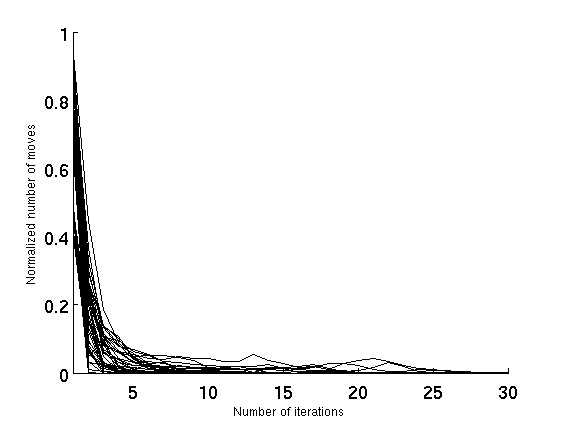
\includegraphics[width = .65\textwidth]{../figures/iterMove.png}
\caption{Number of moved objects per iteration when clustering a variety of datasets with the k-averages algorithm, normalized by the total number of objects to cluster. The datasets used to create this figure are the real-life time series data that we employ for experimental validation evaluated under the Dynamic Time Warping (DTW) similarity measure, \textit{cf.} Section~\ref{sec:experiments}.}
\label{fig:moved}
\end{figure}

\begin{figure}
\center
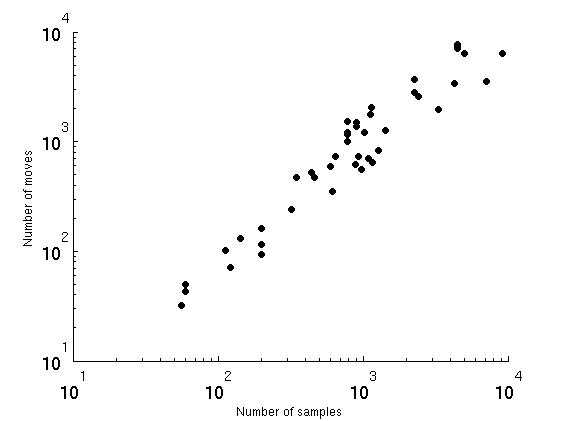
\includegraphics[width = .65\textwidth]{../figures/sampleMove.png}
\caption{Total number of object reallocations over a run of the k-averages algorithm, plotted against the number of objects to be clustered. The datasets used to create this figure are the real-life time series data that we employ for experimental validation, \textit{cf.} Section~\ref{sec:experiments}.}
\label{fig:totalMoved}
\end{figure}

\subsection{Memory access}

The lowered computational costs is also accompanied by a decrease in memory access: as can be seen from Equation~\ref{eq:newSimilNewC}, in order to compute the new object-to-class similarities after moving an object $n$, only line $n$ of the similarity matrix needs to be read. For the remaining of the algorithm, only the (much smaller) object-to-class similarity matrix is used. By contrast, in the case of kernel k-means, the computation of $M_c$ values at each iteration require that the whole similarity matrix be read, which can be a serious performance bottleneck in the case of large object collections.

Moreover, the similarity update function of k-averages, by reading one line of the matrix at a time, presents good data locality properties, which make it play well with standard memory paging strategies.

To illustrate and confirm the theoretical complexity computed here, the next section proposes some performance figures measured on controlled datasets.

\section{Validation}
\label{sec:validation}

In order to reliably compare the clustering quality and execution speed between the two approaches, we have written plain C implementations of Algorithms~\ref{algo:kkmeans_optim} and~\ref{algo:kaverages}, with minimal operational overhead: reading the similarity matrix from a binary file where all matrix values are stored sequentially in standard reading order, line by line, and writing out the result of the clustering as a label text file. Both implementations use reasonably efficient code, but without advanced optimizations or parallel processing.	%% Arshia: remove \footnote{}

The figures presented in this section were obtained on synthetic datasets, created in order to give precise control on the features of the analyzed data: for $n$ points split between $C$ classes, $C$ centroids are generated at random in two dimensional space, and point coordinates are generated following a Gaussian distribution around class centroids. In addition to the numbers of objects and classes, the variance of Gaussian distributions are adjusted to modulate how clearly separable clusters are. Similarities are computed as inverse Euclidean distances between points. %This clearly simplified example is useful as a first control test bench; the next section is dedicated to experiments on more realistic datasets.

\subsection{Reproducibility}

In order to ease reproducibility of the results, the data is taken from a public repository of several benchmark datasets used in academia \cite{UCRArchive} and the code of the proposed method as well as the experimental code used for generated the figures is publicly available\footnote{Available at: \url{https://github.com/mathieulagrange/kaveragePaper}}.


\subsection{Clustering performance}

Several metrics are available to evaluate the performance of a clustering algorithm. The one closest to the actual target application is the raw accuracy, that is the average number of items labeled correctly after an alignment phase of the estimated labeling with the reference \cite{Kuhn1955Hungarian}.

Another metric of choice is the Normalized Mutual Information (NMI) criterion. Based on information theoretic principles, it measures the amount of statistical information shared by the random variables representing the predicted cluster distribution and the reference class distribution of the data points. If $P$ is the random variable denoting the cluster assignments of the points, and $C$ is the random variable denoting the underlying class labels on the points then the NMI measure is defined as:
\[
\textbf{NMI} = \frac{ 2\- I(C;K) }{H(C)+H(K)}
\]

where $I(X;Y)=H(X)−H(X|Y)$ is the mutual information between the random variables $X$ and $Y$, $H(X)$ is the Shannon entropy of $X$,and $H(X|Y)$ is the conditional entropy of $X$ given $Y$. Thanks to the normalization, the metric stays between $0$ and $1$, $1$ indicating a perfect match, and can be used to compare clustering with different numbers of clusters. Interestingly, random prediction gives an NMI close to $0$, whereas the accuracy of a random prediction on a balanced bi-class problem is as high as 50\,\%.

In this paper, for simplicity sake, only the NMI is considered for validations. However, we found that most statements hereafter in terms of performance ranking of the different algorithms still hold while considering the accuracy metric as reference.

\begin{figure}
\center
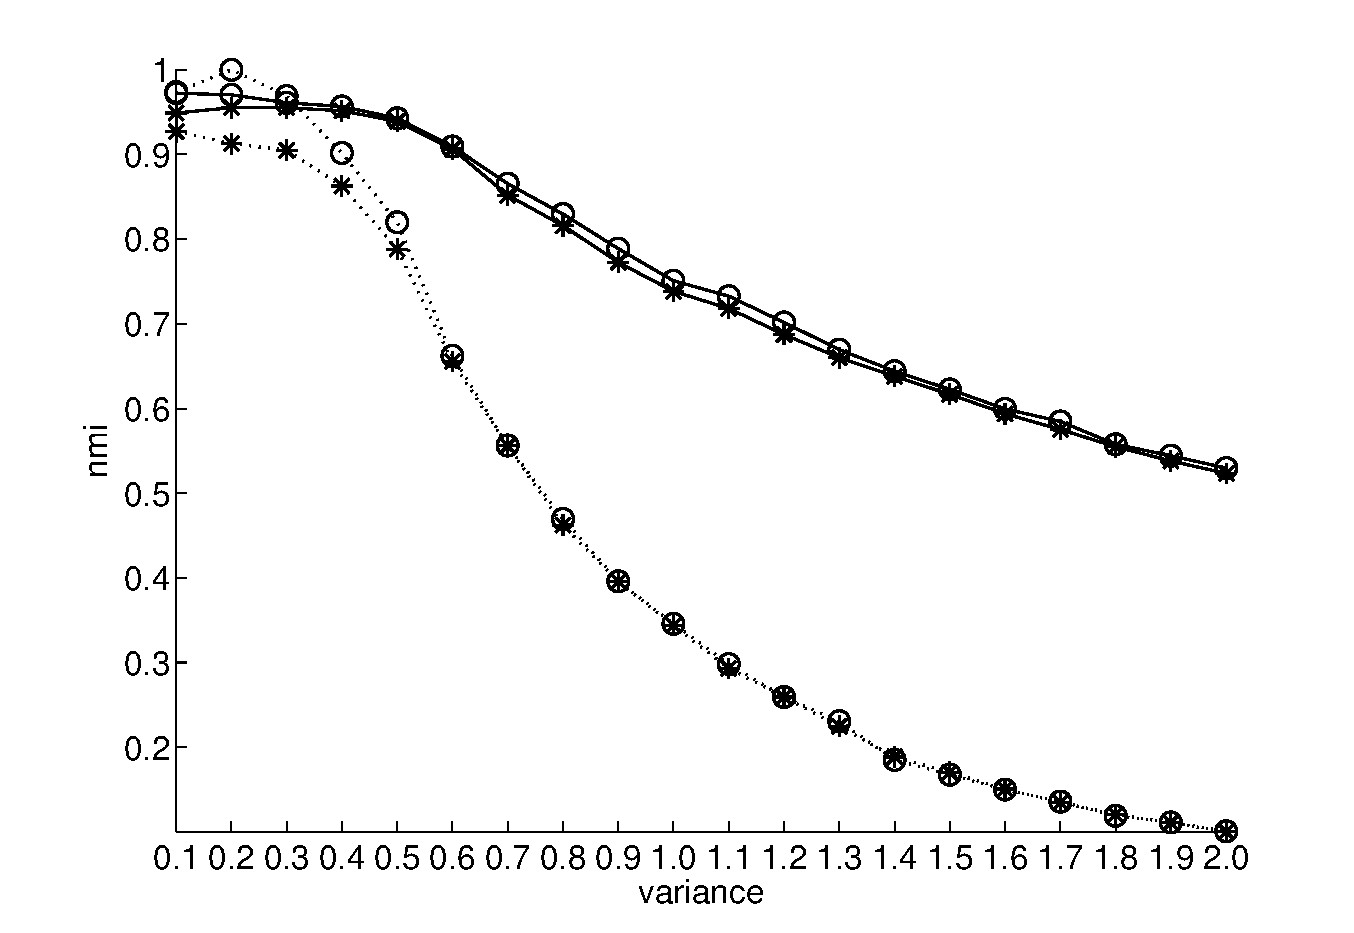
\includegraphics[width=.7\textwidth]{../figures/synthetic.pdf}
\caption{NMI of kernel k-means (*) and k-averages (o) clustering relative to ground truth as a function of the \gl{spread} of those classes for synthetic data sets of 5 and 40 classes, displayed in dashed and solid lines, respectively.}
\label{fig:synth_perf}
\end{figure}

Figure~\ref{fig:synth_perf} presents the quality of clusterings obtained using kernel k-means and k-averages on two series of datasets: one featuring 5 classes, the other 40 classes. On the x-axis is the variance of the Gaussian distribution used to generate the point cloud for each class: the higher that value, the more the classes are spread out and overlap each other, thus making the clustering harder.

The question of choosing the proper number of clusters for a given dataset without \textit{a priori} is a well known and hard problem, and beyond the scope of this article. Therefore, for the purpose of evaluation, clustering is done by requesting a number of clusters equal to the actual number of classes in the dataset. In order to obtain stable and reliable figures, clustering is repeated 500 times with varying initial conditions, \textit{i.e.} the initial assignment of points to clusters is randomly determined, and only the average performance is given. For fairness of comparison, each algorithm is run with the exact same initial assignments.

As can be seen on the figure, in the case of a 5-class problem, k-averages outperforms kernel k-means in the \gl{easy} cases (low class spread), before converging to equivalent results. For the more complex 40-class datasets, k-averages consistently yields a better result than kernel k-means, especially for higher values of the variance. The lower values of NMI for 5-class experiments is in fact an artifact introduced by the normalization of NMI, and is not important here; we only focus, for each series of experiments, on the relative performances of kernel k-means and k-averages.

\subsection{Time efficiency}

Figure~\ref{fig:timing} shows the average time spent by kernel k-means and k-averages to cluster synthetic datasets or varying sizes. As previously, initial conditions on each run are identical for both algorithms. The reported run time is the one measured on a 64 bits Intel$^\circledR$ Core\texttrademark   \, i7 runnning at 3.6 GHz with 32 Gb of RAM and standard Hard Disk Drive (HDD)  operated by standard Linux distribution. For results with 2 GB of RAM, the same machine is used with a memory limitation specified to the kernel at boot time.

\begin{figure}
\center
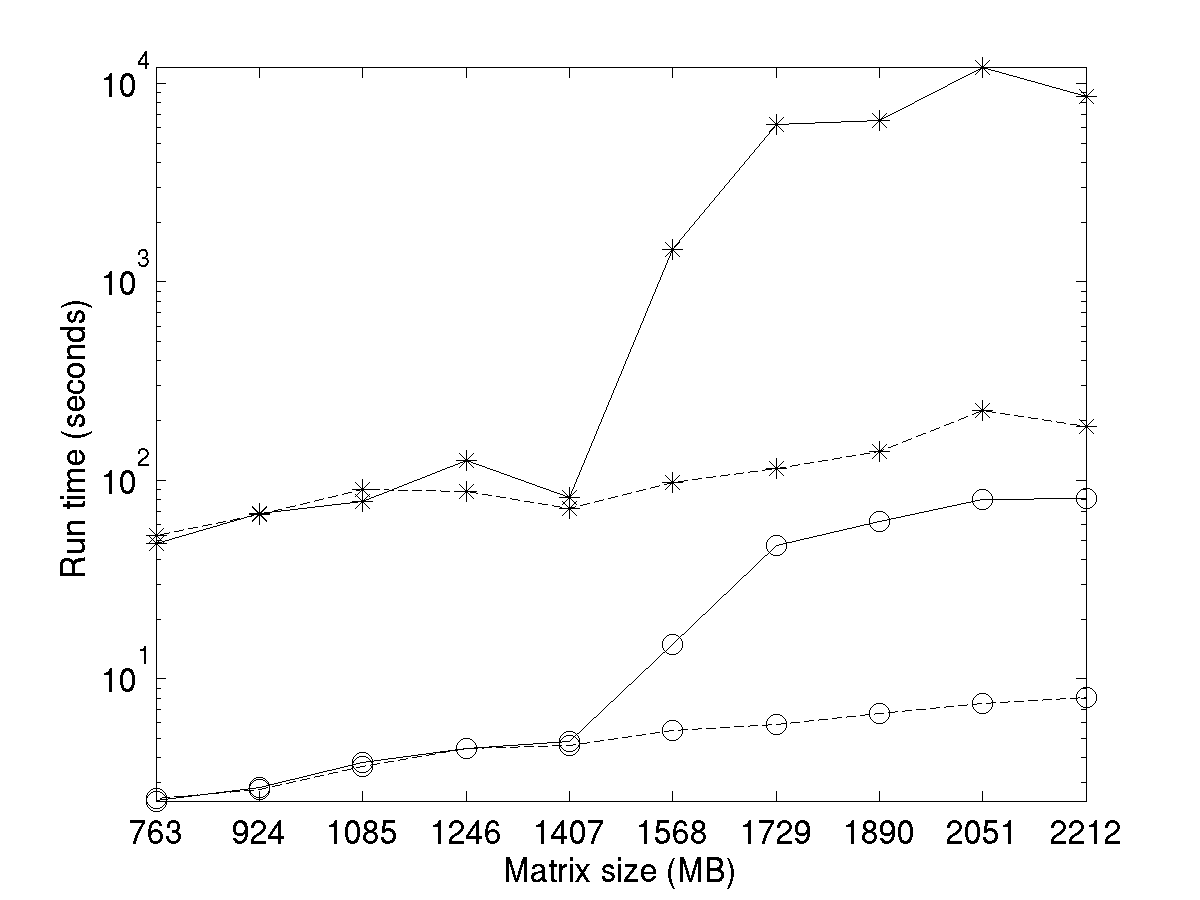
\includegraphics[width= .7\textwidth]{../figures/simpleSwap.png}
\caption{Average computation time of the kernel k-means (*) and kaverages (o) algorithms on computers with 2 GB (solid line) and 32 GB (dashed line) of RAM, respectively. The \gl{running time} axis follows a logarithmic scale.}
\label{fig:timing}
\end{figure}

These figures confirm the theoretical complexity analysis presented in Section~\ref{sec:complexity}: k-averages runs at least 20 times faster on average than kernel k-means in ordinary conditions, when  available memory is not an issue. When the matrix size exceeds what can be stored in RAM and the system has to resort to paged memory, as in the presented experiments when the matrix reaches about 1500MB, both algorithms suffer from a clear performance hit; however, kernel k-means is much more affected, and the difference becomes even more important: with a 2000MB similarity matrix on a memory-limited computer, k-averages runs about 100 times faster than kernel k-means.

Having established the interest of our proposed method relative to kernel k-means on synthetic object collections, we now proceed to a thorough evaluation on real data.

\section{Experiments}
\label{sec:experiments}

In order to demonstrate the usefulness of k-averages when dealing with real data, we have chosen to focus on the clustering of time series as the evaluation task. Time series, even though represented as vectors and therefore suitable for any kinds of norm-based clustering, are best compared with elastic measures \cite{Ding:2008:QMT:1454159.1454226, Wang:2013:ECR:2429736.2429754}, partly due to their varying length. The Dynamic Time Warping (DTW) measure is an elastic measure widely used in many areas since its introduction for spoken word detection \cite{1163055} and has never been challenged for time series mining \cite{conf/kdd/BerndtC94, Rakthanmanon:2013:ABD:2513092.2500489}.

Effective clustering of time series using the DTW measure requires similarity based algorithms such as the k-averages algorithm. With some care, kernel based algorithm can also be considered provided that the resulting similarity matrix is converted into a kernel, \textit{i.e.} the matrix is forced to be semi definite positive, \textit{i.e.} to be a Gram matrix \cite{Lanckriet:2004:LKM:1005332.1005334} in order to guarantee convergence.

\subsection{Datasets}

To compare quality of clusterings obtained by the considered algorithms, we consider a large collection of 43 time series datasets made publicly available by many laboratories worldwide and compiled by Prof. Keogh. Thus, while all the experiments presented here are performed on time series (chosen for being a good example of a data type requiring similarity-based clustering, as opposed to a simple Euclidean approach), the great variety in the sources and semantics of said series (bio-informatics, linguistics, astronomy, gesture modeling, chemistry\ldots{}) gives this validation a wide foundation. Statistics about the morphology of those datasets are summarized in Table~\ref{tab:dbs}. Individual details can be found in Appendix \ref{sec:appendix}.
%In the results described in the next sections, datasets are refered by a numerical id for the sake of brevity; the correspondence between those ids and the actual names of the datasets is shown on Table \ref{didtNoda1}.

\begin{table}
\center
\caption{\label{tab:dbs} Statistics of the datasets. The length of the times series is expressed in samples.}
\begin{tabular}{l|ccc}
& min & average $\pm$ variance & max \\
\hline
number of classes & 2 & 8 $\pm$ 9 & 50 \\
number of time series & 56 & 1626 $\pm$ 2023 & 9236 \\
time series length & 24 & 372 $\pm$ 400 & 1882 \\
\end{tabular}
\end{table}

\subsection{Methods}

Three algorithms are considered: the spectral clustering \cite{von2007tutorial} approach as a high complexity reference, the kernel k-means algorithm implemented as described in Section \ref{sec:kkmeans} and the proposed k-averages algorithm. The spectral clustering algorithm tested here uses the normalization proposed by Jordan and Weiss \cite{ng2002spectral}. This normalization is chosen over no normalization and the Shi and Malik one \cite{shi2000normalized} as it is found to be the best performing in terms of average NMI over all the datasets. The implementation is done using the Matlab programming language. Even though a C implementation would probably be more efficient, we believe that the gain would be low as the main computational load is the diagonalization of the similarity matrix and the k-means clustering of the eigenvectors which are both efficient builtins Matlab functions. The kernel k-means is implemented both in Matlab using the implementation provided by Mo Chen\footnote{Available at: \url{https://fr.mathworks.com/matlabcentral/fileexchange/26182-kernel-kmeans}} and in the C programming language following Algorithm \ref{algo:kkmeans}. The k-averages method is implemented in C following Algorithm \ref{algo:kaverages}.

\subsection{Evaluation Protocol}

For each dataset, since we perform clustering, and not supervised learning, the training and testing data are joined together. DTW similarities are computed using the implementation provided by Prof. Ellis \footnote{Available at: \url{http://www.ee.columbia.edu/~dpwe/resources/matlab/dtw}} with default parameters.

As in our previous experiments with synthetic data, we choose here the normalized mutual information (NMI) as the measure of clustering quality; clustering is done by requesting a number of clusters equal to the actual number of classes in the dataset, and repeated 200 times with varying initial conditions, each algorithm being run with the exact same initial assignments. For the 200 clusterings thus produced, we compute the NMI between them and the ground truth clustering. Average and standard deviation statistics are then computed.

\subsection{Clustering performance}

%% BI-CLASS

\begin{table}
\begin{center}
\caption{NMI (in percents) of clusterings by kernel k-means and k-averages for bi-class datasets.}
\label{tab:results-2}
\begin{tabular}{lccc}
 & spectral clustering & kernel k-means & k-averages \\
\hline
Coffee & 3.4 $\pm$0.0 & 6.9 $\pm$4.1 & \textbf{7.8 $\pm$3.6} \\
ECG200 &  9.9 $\pm$0.0 & \textbf{14.8 $\pm$1.0} & 14.6 $\pm$0.0 \\
ECGFiveDays & 0.1 $\pm$0.0 & \textbf{3.3 $\pm$0.3} & 2.5 $\pm$0.0 \\
Gun\_Point & \textbf{14.8 $\pm$1.3} &  0.0 $\pm$0.0 &  0.0 $\pm$0.0 \\
ItalyPowerDemand & \textbf{1.1} & 0.9 & 0.9 \\
Lighting2 & 4.1 $\pm$0.3 & \textbf{4.9 $\pm$3.7} & 4.3 $\pm$4.2 \\
MoteStrain &  0.0 $\pm$0.0 & \textbf{48.9 $\pm$0.6} & 48.8 $\pm$0.6 \\
SonyAIBORobotSurface &   3.4 $\pm$0.0 & 45.0 $\pm$20.7 & \textbf{45.1 $\pm$20.5} \\
SonyAIBORobotSurfaceII &  2.5 $\pm$0.0 & \textbf{21.4 $\pm$0.0} & \textbf{21.4 $\pm$0.0} \\
TwoLeadECG & \textbf{1.4 $\pm$0.0} & 0.1 $\pm$0.6 & 0.0 $\pm$0.2 \\
wafer & \textbf{0.0} & 0.0 & 0.0 \\
yoga & \textbf{0.5 $\pm$0.0} & 0.2 $\pm$0.1 & 0.2 $\pm$0.1 \\
\end{tabular}
\end{center}
\end{table}

For ease of readability and comparison, the presented results are split into 3 tables. Table~\ref{tab:results-2} lists the results obtained on bi-class datasets, \textit{i.e.} the datasets annotated in terms of presence or absence of a given property; Table~\ref{tab:results-37} concerns the datasets with a small number of classes (from 3 to 7); and Table~\ref{tab:results-8} focuses the datasets with a larger number of classes (from 8 to 50).

For each experiment, the result of the best performing method is marked in bold. The Matlab and C implementations of the kernel k-means algorithm give exactly the same results in terms of NMI, thus only one column is used to display their performance.

 %% 3-7 classes

\begin{table}
\begin{center}
\caption{NMI (in percents) of clusterings by kernel k-means and k-averages for datasets of 3 to 7 classes.}
\label{tab:results-37}
\begin{tabular}{lccc}
 & spectral clustering & kernel k-means & k-averages \\
\hline
Beef & 25.7 $\pm$2.4 & \textbf{35.5 $\pm$2.8} & 34.5 $\pm$2.6 \\
CBF & 11.1 $\pm$0.2 & 41.0 $\pm$8.4 & \textbf{41.0 $\pm$7.0} \\
ChlorineConcentration & \textbf{3.9 $\pm$0.0} & 0.2 $\pm$0.1 & 0.2 $\pm$0.1 \\
CinC\_ECG\_torso & \textbf{37.9 $\pm$0.5} & 24.2 $\pm$1.5 & 24.6 $\pm$1.6 \\
DiatomSizeReduction & 45.3 $\pm$4.2 & \textbf{79.8 $\pm$6.3} & 77.3 $\pm$4.5 \\
FaceFour & 49.8 $\pm$4.6 & 72.2 $\pm$8.4 & \textbf{74.9 $\pm$6.3} \\
Haptics & 3.0 $\pm$0.5 & \textbf{9.7 $\pm$1.3} & 9.4 $\pm$1.2 \\
InlineSkate & 4.6 $\pm$0.5 & 6.3 $\pm$0.7 & \textbf{6.4 $\pm$0.7} \\
Lighting7 & 27.6 $\pm$2.7 & 51.0 $\pm$3.1 & \textbf{51.3 $\pm$1.5} \\
OSULeaf & 22.9 $\pm$0.8 & 22.9 $\pm$2.2 & \textbf{23.0 $\pm$2.5} \\
OliveOil & 10.6 $\pm$2.2 & \textbf{32.4 $\pm$8.6} & 30.6 $\pm$7.8 \\
StarLightCurves & 54.3 $\pm$0.0 & \textbf{60.3 $\pm$0.4} & 60.3 $\pm$0.0 \\
Symbols & 72.0 $\pm$1.7 & 79.1 $\pm$3.8 & \textbf{79.5 $\pm$1.6} \\
Trace & 13.7 $\pm$4.4 & \textbf{54.5 $\pm$5.1} & 54.3 $\pm$6.3 \\
Two\_Patterns &   0.2 $\pm$0.0 & \textbf{10.1 $\pm$10.0} &   8.8 $\pm$9.9 \\
fish & 18.5 $\pm$1.5 & 34.9 $\pm$1.4 & \textbf{35.3 $\pm$1.0} \\
synthetic\_control & 63.0 $\pm$0.7 & 85.3 $\pm$4.9 & \textbf{89.5 $\pm$0.8} \\
\end{tabular}
\end{center}
\end{table}


 %% 8-50 classes

\begin{table}
\begin{center}
\caption{NMI (in percents) of clusterings by kernel k-means and k-averages for datasets of 8 to 50 classes.}
\label{tab:results-8}
\begin{tabular}{lccc}
 & spectral clustering & kernel k-means & k-averages \\
\hline
50words & 46.9 $\pm$1.0 & 69.6 $\pm$0.8 & \textbf{71.7 $\pm$0.6} \\
Adiac & 55.0 $\pm$1.0 & 55.7 $\pm$1.0 & \textbf{58.9 $\pm$0.6} \\
Cricket\_X & 19.2 $\pm$1.1 & 26.1 $\pm$1.8 & \textbf{26.8 $\pm$1.2} \\
Cricket\_Y & 22.8 $\pm$1.3 & 33.0 $\pm$1.5 & \textbf{33.5 $\pm$1.2} \\
Cricket\_Z & 19.2 $\pm$1.3 & 25.5 $\pm$2.2 & \textbf{27.3 $\pm$1.3} \\
FaceAll & 36.4 $\pm$1.2 & \textbf{70.7 $\pm$2.0} & 68.2 $\pm$2.3 \\
FacesUCR & 36.2 $\pm$1.3 & 70.4 $\pm$2.0 & \textbf{71.5 $\pm$1.6} \\
MALLAT & 44.5 $\pm$2.0 & \textbf{90.3 $\pm$4.6} & 89.2 $\pm$3.5 \\
MedicalImages & 19.2 $\pm$1.3 & 29.7 $\pm$1.7 & \textbf{30.4 $\pm$1.6} \\
SwedishLeaf & 48.7 $\pm$1.4 & 70.3 $\pm$1.9 & \textbf{70.8 $\pm$1.4} \\
WordsSynonyms & 31.9 $\pm$1.0 & 50.9 $\pm$1.2 & \textbf{52.1 $\pm$0.8} \\
uWaveGestureLibrary\_X & 24.4 $\pm$0.6 & 46.0 $\pm$1.2 & \textbf{46.2 $\pm$0.5} \\
uWaveGestureLibrary\_Y & 16.2 $\pm$0.3 & 44.9 $\pm$0.4 & \textbf{45.0 $\pm$0.2} \\
uWaveGestureLibrary\_Z & 23.2 $\pm$0.6 & \textbf{42.9 $\pm$0.7} & 42.6 $\pm$0.5 \\
\end{tabular}
\end{center}
\end{table}

A first observation is that the spectral clustering algorithm only performs favorably for 2 of the 43 dataset. Also, most of the bi-class problems (Table~\ref{tab:results-2}) do not seem to lend themselves well to this kind of approach: kernel k-means and k-averages produce quasi-identical results, poor in most cases. Concerning the medium numbers of classes (Table~\ref{tab:results-37}), k-averages performs best for 8 datasets out of 17. For the larger numbers of classes (Table~\ref{tab:results-8}), k-averages performs best for 11 datasets out of 14.

Considering the standard deviation over the several runs of the algorithm with different initialization is helpful to study the sensitivity of the algorithm to its initialization and thus its tendency to be stuck into local minima. For most datasets, the standard deviation of the k-averages algorithm is smaller than the one of the kernel k-means one and thus seems experimentally more robust.

\subsection{Efficiency}

Computation time displayed in Tables \ref{tab:resultSpeed-2}, \ref{tab:resultSpeed-37}, and \ref{tab:resultSpeed-8} is the average duration over 100 runs on a single core with no parallelization capabilities. For every datasets, the spectral clustering approach is the more time consuming due to the diagonalization of the matrix which is of $O(N^3)$. For the kernel k-means algorithm, the C implementation is most of the time more efficient than the Matlab implementation. The k-average algorithm is more efficient for 46 datasets out of the 47 by close to an order of magnitude for the larger datasets.

\begin{table}
\begin{center}
\caption{Computation time (in seconds) for several implementations of the evaluated clustering algorithms for datasets of 2 classes.}
\label{tab:resultSpeed-2}
\begin{tabular}{lcccc}
 & \multicolumn{2}{c}{Matlab} & \multicolumn{2}{c}{C} \\
 & spectral clustering & kk-means & kk-means & k-averages \\
\hline
Coffee & 0.02 & 0.00 & \textbf{0.00} & 0.00 \\
ECG200 & 0.03 & 0.00 & 0.00 & \textbf{0.00} \\
ECGFiveDays & 0.13 & 0.10 & 0.06 & \textbf{0.01} \\
Gun\_Point & 0.02 & 0.00 & 0.00 & \textbf{0.00} \\
ItalyPowerDemand & 0.20 & 0.07 & 0.05 & \textbf{0.01} \\
Lighting2 & 0.02 & 0.00 & 0.00 & \textbf{0.00} \\
MoteStrain & 0.33 & 0.11 & 0.08 & \textbf{0.01} \\
SonyAIBORobotSurface & 0.09 & 0.02 & 0.01 & \textbf{0.00} \\
SonyAIBORobotSurfaceII & 0.09 & 0.01 & 0.02 & \textbf{0.01} \\
TwoLeadECG & 0.13 & 0.16 & 0.10 & \textbf{0.02} \\
wafer & 19.62 &  0.72 &  1.04 & \textbf{ 0.39} \\
yoga & 3.55 & 0.80 & 0.66 & \textbf{0.10} \\
\end{tabular}
\end{center}
\end{table}

\begin{table}
\begin{center}
\caption{Computation time (in seconds) for several implementations of the evaluated clustering algorithms for datasets of 3 to 7 classes.}
\label{tab:resultSpeed-37}
\begin{tabular}{lcccc}
  & \multicolumn{2}{c}{Matlab} & \multicolumn{2}{c}{C} \\
  & spectral clustering & kk-means & kk-means & k-averages \\
\hline
Beef & 0.02 & 0.00 & 0.00 & \textbf{0.00} \\
CBF & 0.17 & 0.08 & 0.05 & \textbf{0.01} \\
ChlorineConcentration & 7.15 & 2.74 & 2.09 & \textbf{0.23} \\
CinC\_ECG\_torso & 0.55 & 0.31 & 0.16 & \textbf{0.04} \\
DiatomSizeReduction & 0.04 & 0.01 & 0.00 & \textbf{0.00} \\
FaceFour & 0.02 & 0.00 & 0.00 & \textbf{0.00} \\
Haptics & 0.07 & 0.04 & 0.01 & \textbf{0.01} \\
InlineSkate & 0.12 & 0.08 & 0.03 & \textbf{0.01} \\
Lighting7 & 0.04 & 0.01 & 0.00 & \textbf{0.00} \\
OSULeaf & 0.08 & 0.04 & 0.01 & \textbf{0.00} \\
OliveOil & 0.03 & 0.00 & 0.00 & \textbf{0.00} \\
StarLightCurves & 34.16 &  4.69 &  6.21 & \textbf{ 0.91} \\
Symbols & 0.26 & 0.15 & 0.06 & \textbf{0.02} \\
Trace & 0.02 & 0.01 & 0.00 & \textbf{0.00} \\
Two\_Patterns & 11.99 &  3.99 &  3.71 & \textbf{ 0.40} \\
fish & 0.06 & 0.02 & 0.01 & \textbf{0.00} \\
synthetic\_control & 0.09 & 0.03 & 0.01 & \textbf{0.01} \\
\end{tabular}
\end{center}
\end{table}


 %% 8-50 classes

\begin{table}
\begin{center}
\caption{Computation time (in seconds) for several implementations of the evaluated clustering algorithms for datasets of 8 to 50 classes.}
\label{tab:resultSpeed-8}
\begin{tabular}{lcccc}
  & \multicolumn{2}{c}{Matlab} & \multicolumn{2}{c}{C} \\
  & spectral clustering & kk-means & kk-means & k-averages \\
\hline
50words & 0.89 & 0.19 & 0.05 & \textbf{0.03} \\
Adiac & 0.49 & 0.16 & 0.05 & \textbf{0.03} \\
Cricket\_X & 0.24 & 0.10 & 0.05 & \textbf{0.02} \\
Cricket\_Y & 0.22 & 0.09 & 0.05 & \textbf{0.02} \\
Cricket\_Z & 0.22 & 0.09 & 0.04 & \textbf{0.02} \\
FaceAll & 2.08 & 0.78 & 0.40 & \textbf{0.11} \\
FacesUCR & 2.21 & 0.75 & 0.41 & \textbf{0.12} \\
MALLAT & 2.23 & 0.47 & 0.29 & \textbf{0.12} \\
MedicalImages & 0.42 & 0.24 & 0.12 & \textbf{0.04} \\
SwedishLeaf & 0.56 & 0.22 & 0.11 & \textbf{0.04} \\
WordsSynonyms & 0.44 & 0.16 & 0.08 & \textbf{0.03} \\
uWaveGestureLibrary\_X & 8.60 & 5.15 & 3.82 & \textbf{0.44} \\
uWaveGestureLibrary\_Y & 8.94 & 4.48 & 2.65 & \textbf{0.45} \\
uWaveGestureLibrary\_Z & 8.53 & 4.00 & 2.89 & \textbf{0.47} \\
\end{tabular}
\end{center}
\end{table}


\subsection{Overall results}

To conclude on the performance of the evaluated algorithms on real datasets, Table \ref{tab:resultAverage} displays the NMI and computation time averaged over the 47 datasets. The k-averages method marginally improve the clustering accuracy compared to the kernel k-means approach by using less time to compute.

\begin{table}
\begin{center}
\caption{Performances averaged over the 47 datasets. The NMI is expressed in percents and the computation time in seconds.}
\label{tab:resultAverage}
\begin{tabular}{lcccc}
  & \multicolumn{2}{c}{Matlab} & \multicolumn{2}{c}{C} \\
  & spectral clustering & kk-means & kk-means & k-averages \\
\hline
nmi (\%) & 22.1 & 36.6 & 36.6 & \textbf{36.8} \\
computation time & 2.678 & 0.723 & 0.590 & \textbf{0.096} \\
\end{tabular}
\end{center}
\end{table}

\section{Conclusion}

We have presented k-averages, an iterative flat clustering algorithm that operates on arbitrary similarity matrices by explicitly and directly aiming to optimize the average intra-class similarity. Having established the mathematical foundation of our proposal, including guaranteed convergence, we have thoroughly compared it with widely used standard methods: the kernel k-means and the spectral clustering techniques. We show that the k-averages algorithm converges much faster (20 times faster under ordinary conditions) and leads to equivalent or better clustering results for the task of clustering both synthetic data and realistic times series taken from a wide variety of sources, while also being more computationally efficient and more sparing in memory use.

%The linear updates and compensated memory access of the proposed k-average method also provide great potentials for online clustering methods, where time-series data arrive incrementally into the system, and where classes and clusters should be most often reallocated. Explicit reallocation considerations proposed in this paper pave the way for robust online clustering methods that shall be further pursued.

%Implementations of k-averages in Matlab and C are freely available as mature code ready for general use, at <url>. That repository also contains the reference C implementation of kernel k-means which we have used for the experiments reported in this article.



%\bibliographystyle{plos2015}
%\bibliography{../bib}

\section*{Acknowledgments}

The authors would like to acknowledge support for this project
from ANR project Houle (grant ANR-11-JS03-005-01) and ANR project Cense (grant ANR-16-CE22-0012).

\nolinenumbers

% Either type in your references using
% \begin{thebibliography}{}
% \bibitem{}
% Text
% \end{thebibliography}
%
% or
%
% Compile your BiBTeX database using our plos2015.bst
% style file and paste the contents of your .bbl file
% here. See http://journals.plos.org/plosone/s/latex for
% step-by-step instructions.
%
\begin{thebibliography}{10}

  \bibitem{jain2010data}
  Jain AK.
  \newblock Data clustering: 50 years beyond K-means.
  \newblock Pattern Recognition Letters. 2010;31:651--666.

  \bibitem{steinbach2000comparison}
  Steinbach M, Karypis G, Kumar V, et~al.
  \newblock A comparison of document clustering techniques.
  \newblock In: KDD workshop on text mining. vol. 400. Boston; 2000. p. 525--526.

  \bibitem{thalamuthu2006evaluation}
  Thalamuthu A, Mukhopadhyay I, Zheng X, Tseng GC.
  \newblock Evaluation and comparison of gene clustering methods in microarray
    analysis.
  \newblock Bioinformatics. 2006;22:2405--2412.

  \bibitem{macQueenBsmsp67}
  MacQueen JB.
  \newblock {Some Methods for classification and Analysis of Multivariate
    Observations}.
  \newblock In: Proc. of Berkeley Symposium on Mathematical Statistics and
    Probability; 1967.

  \bibitem{Banerjee:2005:CBD:1046920.1194902}
  Banerjee A, Merugu S, Dhillon IS, Ghosh J.
  \newblock Clustering with Bregman Divergences.
  \newblock J Mach Learn Res. 2005;6:1705--1749.

  \bibitem{Dhillon:2003:DIT:944919.944973}
  Dhillon IS, Mallela S, Kumar R.
  \newblock A Divisive Information Theoretic Feature Clustering Algorithm for
    Text Classification.
  \newblock J Mach Learn Res. 2003;3:1265--1287.

  \bibitem{linde:algorithm}
  Linde Y, Buzo A, Gray RM.
  \newblock An Algorithm for Vector Quantizer Design.
  \newblock IEEE Transactions on Communications. 1980;28:84--95.

  \bibitem{KaufmanRousseeuw90}
  Kaufman L, Rousseeuw PJ.
  \newblock Finding groups in data: an introduction to cluster analysis.
  \newblock New York: John Wiley and Sons; 1990.

  \bibitem{Ng:1994:EEC:645920.672827}
  Ng RT, Han J.
  \newblock Efficient and Effective Clustering Methods for Spatial Data Mining.
  \newblock In: Proceedings of the 20th International Conference on Very Large
    Data Bases. VLDB '94. San Francisco, CA, USA: Morgan Kaufmann Publishers
    Inc.; 1994. p. 144--155.

  \bibitem{Duda01}
  Duda RO, Hart PE, Stork DG.
  \newblock Pattern Classification (2nd Ed).
  \newblock Wiley; 2001.

  \bibitem{Vapnik:1995:NSL:211359}
  Vapnik VN.
  \newblock The Nature of Statistical Learning Theory.
  \newblock New York, NY, USA: Springer-Verlag New York, Inc.; 1995.

  \bibitem{Girolami:2002:MKC:2325785.2326903}
  Girolami M.
  \newblock Mercer Kernel-based Clustering in Feature Space.
  \newblock IEEE Transactions on Neural Network. 2002;13(3):780--784.
  \newblock doi:{10.1109/TNN.2002.1000150}.

  \bibitem{Dhillon:2007:WGC:1313055.1313291}
  Dhillon IS, Guan Y, Kulis B.
  \newblock Weighted Graph Cuts Without Eigenvectors A Multilevel Approach.
  \newblock IEEE Trans Pattern Anal Mach Intell. 2007;29(11):1944--1957.
  \newblock doi:{10.1109/TPAMI.2007.1115}.

  \bibitem{von2007tutorial}
  Von~Luxburg U.
  \newblock A tutorial on spectral clustering.
  \newblock Statistics and computing. 2007;17(4):395--416.

  \bibitem{shi2000normalized}
  Shi J, Malik J.
  \newblock Normalized cuts and image segmentation.
  \newblock IEEE Transactions on pattern analysis and machine intelligence.
    2000;22(8):888--905.

  \bibitem{Roth:2003:OCP:960254.960291}
  Roth V, Laub J, Kawanabe M, Buhmann JM.
  \newblock Optimal Cluster Preserving Embedding of Nonmetric Proximity Data.
  \newblock IEEE Trans Pattern Anal Mach Intell. 2003;25(12):1540--1551.
  \newblock doi:{10.1109/TPAMI.2003.1251147}.

  \bibitem{Chitta:2011:AKK:2020408.2020558}
  Chitta R, Jin R, Havens TC, Jain AK.
  \newblock Approximate Kernel K-means: Solution to Large Scale Kernel
    Clustering.
  \newblock In: Proceedings of the 17th ACM SIGKDD International Conference on
    Knowledge Discovery and Data Mining. KDD '11. New York, NY, USA: ACM; 2011.
    p. 895--903.

  \bibitem{1047453}
  Zhang R, Rudnicky AI.
  \newblock A large scale clustering scheme for kernel K-Means.
  \newblock In: Pattern Recognition, 2002. Proceedings. 16th International
    Conference on. vol.~4; 2002. p. 289--292 vol.4.

  \bibitem{bradley98scaling}
  Bradley PS, Fayyad UM, Reina C.
  \newblock Scaling Clustering Algorithms to Large Databases.
  \newblock In: Knowledge Discovery and Data Mining; 1998. p. 9--15.

  \bibitem{Kulis2008}
  Kulis B, Basu S, Dhillon I, Mooney R.
  \newblock {Semi-supervised graph clustering: a kernel approach}.
  \newblock Machine Learning. 2008;74(1):1--22.
  \newblock doi:{10.1007/s10994-008-5084-4}.

  \bibitem{UCRArchive}
  Chen Y, Keogh E, Hu B, Begum N, Bagnall A, Mueen A, et~al.. The UCR Time Series
    Classification Archive; 2015.

  \bibitem{Kuhn1955Hungarian}
  Kuhn HW.
  \newblock {The Hungarian Method for the Assignment Problem}.
  \newblock Naval Research Logistics Quarterly. 1955;2(1--2):83--97.
  \newblock doi:{10.1002/nav.3800020109}.

  \bibitem{Ding:2008:QMT:1454159.1454226}
  Ding H, Trajcevski G, Scheuermann P, Wang X, Keogh E.
  \newblock Querying and Mining of Time Series Data: Experimental Comparison of
    Representations and Distance Measures.
  \newblock Proc VLDB Endowment. 2008;1(2):1542--1552.
  \newblock doi:{10.14778/1454159.1454226}.

  \bibitem{Wang:2013:ECR:2429736.2429754}
  Wang X, Mueen A, Ding H, Trajcevski G, Scheuermann P, Keogh E.
  \newblock Experimental Comparison of Representation Methods and Distance
    Measures for Time Series Data.
  \newblock Data Mining Knowledge Discovery. 2013;26(2):275--309.
  \newblock doi:{10.1007/s10618-012-0250-5}.

  \bibitem{1163055}
  Sakoe H, Chiba S.
  \newblock Dynamic programming algorithm optimization for spoken word
    recognition.
  \newblock IEEE Transactions on Acoustics, Speech and Signal Processing.
    1978;26(1):43--49.
  \newblock doi:{10.1109/TASSP.1978.1163055}.

  \bibitem{conf/kdd/BerndtC94}
  Berndt DJ, Clifford J.
  \newblock Using Dynamic Time Warping to Find Patterns in Time Series.
  \newblock In: Fayyad UM, Uthurusamy R, editors. KDD Workshop. AAAI Press; 1994.
    p. 359--370.

  \bibitem{Rakthanmanon:2013:ABD:2513092.2500489}
  Rakthanmanon T, Campana B, Mueen A, Batista G, Westover B, Zhu Q, et~al.
  \newblock Addressing Big Data Time Series: Mining Trillions of Time Series
    Subsequences Under Dynamic Time Warping.
  \newblock ACM Trans Knowl Discov Data. 2013;7(3):10:1--10:31.
  \newblock doi:{10.1145/2500489}.

  \bibitem{Lanckriet:2004:LKM:1005332.1005334}
  Lanckriet GRG, Cristianini N, Bartlett P, Ghaoui LE, Jordan MI.
  \newblock Learning the Kernel Matrix with Semidefinite Programming.
  \newblock J Mach Learn Res. 2004;5:27--72.

  \bibitem{ng2002spectral}
  Ng AY, Jordan MI, Weiss Y.
  \newblock On spectral clustering: Analysis and an algorithm.
  \newblock In: Advances in neural information processing systems; 2002. p.
    849--856.

  \end{thebibliography}


\appendix

\section{Description of the datasets}
\label{sec:appendix}

\begin{table} [h!]
\begin{center}
\caption{Description of the time series datasets used for evaluation.}
\label{didtNoda1}
\small
 \setlength{\tabcolsep}{.16667em}
\begin{tabular}{lcc}
name & number of classes & number of samples \\
\hline
50words & 50 &  905 \\
Adiac & 37 &  781 \\
Beef &  5 &   60 \\
CBF  &  3 &  930 \\
ChlorineConcentration  &  3 & 4307 \\
CinC\_ECG\_torso  &  4 & 1420 \\
Coffee  &  2 &   56 \\
Cricket\_X  & 12 &  780 \\
Cricket\_Y  & 12 &  780 \\
Cricket\_Z  & 12 &  780 \\
DiatomSizeReduction  &  4 &  322 \\
ECG200  &  2 &  200 \\
ECGFiveDays  &  2 &  884 \\
FaceAll &  14 & 2250 \\
FaceFour &   4 &  112 \\
FacesUCR &  14 & 2250 \\
Gun\_Point &   2 &  200 \\
Haptics &   5 &  463 \\
InlineSkate  &  7 &  650 \\
ItalyPowerDemand  &  2 & 1096 \\
Lighting2  &  2 &  121 \\
Lighting7  &  7 &  143 \\
MALLAT  &  8 & 2400 \\
MedicalImages  & 10 & 1141 \\
MoteStrain  &  2 & 1272 \\
OSULeaf &   6 &  442 \\
OliveOil &   4 &   60 \\
SonyAIBORobotSurface &   2 &  621 \\
SonyAIBORobotSurfaceII &   2 &  980 \\
StarLightCurves  &  3 & 9236 \\
SwedishLeaf & 15 & 1125 \\
Symbols  &  6 & 1020 \\
Trace &   4 &  200 \\
TwoLeadECG  &  2 & 1162 \\
Two\_Patterns  &  4 & 5000 \\
WordsSynonyms  & 25 &  905 \\
fish  &  7 &  350 \\
synthetic\_control  &  6 &  600 \\
uWaveGestureLibrary\_X  &  8 & 4478 \\
uWaveGestureLibrary\_Y  &  8 & 4478 \\
uWaveGestureLibrary\_Z  &  8 & 4478 \\
wafer  &  2 & 7164 \\
yoga  &  2 & 3300 \\
\end{tabular}
\end{center}
\end{table}

\end{document}
